\documentclass[12pt]{article}
\usepackage[utf8]{inputenc}

\usepackage{lmodern}

\usepackage{enumitem}
\usepackage[margin=2cm]{geometry}

\usepackage{amsmath, amsfonts, amssymb}
\usepackage{graphicx}
%\usepackage{subfigure}
\usepackage{tikz}
\usepackage{pgfplots}
\usepackage{multicol}

\usepackage{comment}
\usepackage{url}
\usepackage{calc}
\usepackage{subcaption}
\usepackage[indent=0pt]{parskip}
\usepackage{animate}

\usepackage{array}
\usepackage{blkarray,booktabs, bigstrut}
\usepackage{bigints}

\pgfplotsset{compat=1.16}

% MATH commands
\newcommand{\ga}{\left\langle}
\newcommand{\da}{\right\rangle}
\newcommand{\oa}{\left\lbrace}
\newcommand{\fa}{\right\rbrace}
\newcommand{\oc}{\left[}
\newcommand{\fc}{\right]}
\newcommand{\op}{\left(}
\newcommand{\fp}{\right)}

\newcommand{\bi}{\mathbf{i}}
\newcommand{\bj}{\mathbf{j}}
\newcommand{\bk}{\mathbf{k}}
\newcommand{\bF}{\mathbf{F}}

\newcommand{\mR}{\mathbb{R}}

\newcommand{\ra}{\rightarrow}
\newcommand{\Ra}{\Rightarrow}

\newcommand{\sech}{\mathrm{sech}\,}
\newcommand{\csch}{\mathrm{csch}\,}
\newcommand{\curl}{\mathrm{curl}\,}
\newcommand{\dive}{\mathrm{div}\,}

\newcommand{\ve}{\varepsilon}
\newcommand{\spc}{\vspace*{0.5cm}}

\DeclareMathOperator{\Ran}{Ran}
\DeclareMathOperator{\Dom}{Dom}

\newcommand{\exo}[1]{\noindent\textcolor{red}{\fbox{\textbf{Problem {#1}}}\hrulefill}\\\\ }
\newcommand{\qu}[4]{\noindent\textcolor{#4}{\fbox{\textbf{Section {#1} | Problem {#2}}} \hrulefill{{\fbox{\textbf{{#3} Points}}}}\\}}

\newcommand{\semester}{Fall 2023}

\newcommand{\CVup}{%

\begin{tikzpicture}
\draw[black, <->, >=latex] (-0.33, 0.5) .. controls (-0.125, 0) and (0.125, 0) .. (0.33, 0.5);
\end{tikzpicture}}

\newcommand{\CVupInc}{%
\begin{tikzpicture}
\draw[black, ->, >=latex] (0,0) .. controls (0.2, 0) and (0.4, 0.2) .. (0.5, 0.5);
\end{tikzpicture}}

\newcommand{\CVupDec}{%
\begin{tikzpicture}[rotate=270]
\draw[black, ->, >=latex] (0,0) .. controls (0.2, 0) and (0.4, 0.2) .. (0.5, 0.5);
\end{tikzpicture}}

\newcommand{\CVdown}{%
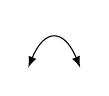
\begin{tikzpicture}
\draw[black, <->, >=latex] (-0.33, -0.5) .. controls (-0.125, 0) and (0.125, 0) .. (0.33, -0.5);
\end{tikzpicture}}

\newcommand{\CVdownInc}{%
\begin{tikzpicture}
\draw[black, ->, >=latex] (-0.5, -0.5) .. controls (-0.5, -0.3) and (-0.5, -0.1) .. (0,0);
\end{tikzpicture}}

\newcommand{\CVdownDec}{%
\begin{tikzpicture}[rotate=-90]
\draw[black, ->, >=latex] (-0.5, -0.5) .. controls (-0.5, -0.3) and (-0.5, -0.1) .. (0,0);
\end{tikzpicture}}

\begin{document}
	\noindent \hrulefill \\
	MATH-244 \semester \hfill Practice Problems Solutions\\
	Section 15.6 \hfill Pierre-Olivier Paris{\'e} \\\vspace*{-1cm}
	
	\noindent\hrulefill
	
	\spc	

	\exo{4}
	\\
	We have
		\begin{align*}
		\int_0^1 \int_y^{2y} \int_0^{x + y} 6xy \, dz dx dy &= \int_0^1 \int_y^{2y} 6 xy (x + y) \, dx dy \\
		&= \int_0^1 \int_y^{2y} 6x^2y + 6xy^2 \, dx dy \\
		&= \int_0^1 \left. (2x^3 y + 3 x^2y^2 ) \right|_{x = y}^{x = 2y} \, dy \\
		&= \int_0^1 (16y^4 + 12y^4) - (2y^4 + 3y^4) \, dy \\
		&= \int_0^1 23 y^4 \, dy \\
		&= \frac{23}{5} .
		\end{align*}
	
	\spc 
	
	\exo{12}
	\\
	The solid is described in the following way
		\begin{align*}
		E = \{ (x, y , z) \, : \, 0 \leq x \leq \pi \text{, } 0 \leq y \leq \pi - x \text{, } 0 \leq z \leq x \} .
		\end{align*}
	So,
		\begin{align*}
		\iiint_E \sin y \, dV = \int_0^\pi \int_0^{\pi - x} \int_0^x \sin y \, dz dy dx &= \int_0^\pi x \left. (-\cos y) \right|_{y =0}^{y = \pi - x} \, dx \\
		&= \int_0^\pi -x (1 + \cos (\pi - x)) \, dx .
		\end{align*}
	After an integration by parts, we get
		\begin{align*}
		\iiint_E \sin y \, dV = -2 - \pi^2/2 \approx -6.9348 .
		\end{align*}
	
	\spc 
	
	\exo{20}
	\\
	So we have $x^2 + z^2 \leq y \leq 8 - x^2 - z^2$. We have to intersect the two surfaces to find the domain of integration in the $XZ$-plane. Equating both equations for the surfaces to $y$, we get
		\begin{align*}
		x^2 + z^2 = 8 - x^2 - z^2 \iff x^2 + z^2 = 4 .
		\end{align*}
	So the domain is a circle of radius $2$. Thus, the volume will be given by
		\begin{align*}
		V = \iiint_E \, dV = \int_0^{2\pi} \int_0^{2} \int_{r^2}^{8 - r^2} \, dy r dr d\theta
		\end{align*}
	where we describe the domain in the $XZ$-plane in polar coordinates. So
		\begin{align*}
		V = 2\pi \int_0^2 (8 - 2r^2) r \, dr = 2\pi  \int_0^4 u \, du = 16 \pi .
		\end{align*}
	
	\spc 
	
	\exo{34}
	\\
	We have 
		\begin{align*}
		E = \{ (x, y, z) \, : \, 0 \leq x \leq 1 \text{, } 0 \leq y \leq 1 - x \text{, } 0 \leq z \leq 1 - x^2 \} .
		\end{align*}
		
	The orders we would like are $dz dy dx$, $dy dx dz$, $dx dy dz$, $dz dx dy$, $dx dz dy$.
	
	\begin{enumerate}
	\item $\mathbf{dzdydx}$. Since the bounds depend only on $x$, we can interchange without problems:
		\begin{align*}
		\int_0^1 \int_{0}^{1 - x} \int_0^{1 - x^2} f(x, y, z) \, dz dy dx .
		\end{align*}
	\item $\mathbf{dydxdz}$. We have to look into the $XZ$-plane and interchange. The region in this plane are bounded by the curves $x = 0$, $x = 1$, $z = 0$ and $z = 1-x^2$ and looks like this:
		\begin{figure}[h]
		\centering
		\includegraphics[scale=0.5]{problem64-dydxdz.png}
		\end{figure}
	So, by seeing this region as a type two, we get $0 \leq x \leq \sqrt{1 - z}$ and $0 \leq z \leq 1$. We then obtain
		\begin{align*}
		\int_0^1 \int_0^{\sqrt{1- z}} \int_0^{1-x} f(x, y ,z) \, dy dx dz .
		\end{align*}
	\item $\mathbf{dxdydz}$. We have to look into the $XY$-plane. We see that $0 \leq x \leq \sqrt{1 - z}$ and $0 \leq y \leq 1 - x$. Here, $z$ is considered as a number which is fixed. If we see this domain as a type II (to interchange the $x$ and the $y$), we have to deal with two pieces:
		\begin{itemize}
		\item $0 \leq y \leq 1 - \sqrt{1-z}$, then $0 \leq x \leq \sqrt{1 - z}$.
		\item $1 - \sqrt{1 - z} \leq y \leq 1$, then $0 \leq x \leq 1 - y$.
		\end{itemize}
	So the integral becomes
		\begin{align*}
		\int_0^1 \Big( \int_0^{1-\sqrt{1-z}} \int_0^{\sqrt{1 - z}} f(x, y, z) \, dx dy + \int_{1 - \sqrt{1-z}}^1 \int_0^{1-y} f(x, y, z) \, dx dy \Big) \, dz .
		\end{align*}
	\item $\mathbf{dz dx dy}$. We look in the $XY$-plane in the original configuration. From the bounds in the integrals in $x$ and $y$, the region in the $XY$-plane is bounded by the curves $x = 0$, $x = 1$, $y = 0$ and $y = 1-x$. So we interchange easily and get $0 \leq x \leq 1 - y$ and $0 \leq y \leq 1$ to get
		\begin{align*}
		\int_0^1 \int_0^{1-y} \int_0^{1-x^2} f(x, y, z) \, dz dx dy .
		\end{align*}
	\item $\mathbf{dx dz dy}$. We look at the bounds in $x$ and $z$. We see these bounds give a region bounded by $x = 0$, $x = 1-y$, $z = 0$, and $z = 1-x^2$. Again, we have to split into two cases:
		\begin{itemize}
		\item $0 \leq z \leq 1 - (1-y)^2$, $0 \leq x \leq 1 - y$;
		\item $1 - (1 -y)^2 \leq z \leq 1$, $0 \leq x \leq \sqrt{1 - z}$.
		\end{itemize}
	So the integral in this final order looks like
		\begin{align*}
		\int_0^1 \Big( \int_0^{1 - (1-y)^2} \int_0^{1 - y} f(x, y, z) \, dx dz + \int_{1- (1-y)^2}^1 \int_0^{\sqrt{1 - z}} f(x, y, z) \, dx dz \Big) dy .
		\end{align*}
	\end{enumerate}

\end{document}